%%%%%%%%%%%%%%%%%%%%%%%%%%%%%%%%%%%%%%%%%%%%%%
%% Modèle de rapport pédagogique v3
%%
%% Vincent Labatut 2014-2016
%%
%% v1   - 10/2014 : forme de rapport très différente
%% v2   - 02/2015 : modèle complètement refait
%% v2.1 - 03/2015 : définition de la page de titre
%% v2.2 - 03/2015 : correction de quelques bugs
%% v2.3 - 04/2015 : page de titre complétée (date, adresse postale, long titre)
%% v2.4 - 12/2015 : diverses modifications du contenu du document
%% v3   - 01/2016 : définition de la classe latex, correction de quelques erreurs dans le texte
%%
%% À faire :
%%	- options pour les différentes toc
%%  - titre sur plusieurs lignes dans page de garde
%%%%%%%%%%%%%%%%%%%%%%%%%%%%%%%%%%%%%%%%%%%%%%
\documentclass{ceri}

% le caractère '%' permet d'insérer des commentaires, qui seront
% ignorés par le compilateur


%%%%%%%%%%%%%%%%%%%%%%%%%%%%%%%%%%%%%%%%%%%%%%%%%%%
%% Informations générales
%%%%%%%%%%%%%%%%%%%%%%%%%%%%%%%%%%%%%%%%%%%%%%%%%%%
%TODO Titre du document, à adapter
\title{Titre du document}    

%TODO Liste des auteurs
\author{
	Prénom1 Nom1, 
	Prénom2 Nom2 \&
	Prénom3 Nom3
} 

%TODO UE concernée par le rapport (à modifier)
% exemples : UE 
\classname{Nom de l'UE}

%TODO formation concernée : à compléter
% exemples : Licence Informatique, Master Informatique
\formation{Nom de la formation}

%TODO parcours ou spécialité de la formation
% exemples pour la licence : Parcours Systèmes et Réseaux Informatiques, Parcours Ingénierie Logicielle
% exemples pour le master : Spécialité Ingénierie du Logiciel pour la Société Numérique, Spécialité Réseaux Informatiques et Services Mobiles
\parcours{Nom du parcours/spécialité}

\begin{document}

% création de la page de titre
\maketitle

% création de la table des matières
\MyToc

% Justification moins stricte : des mots ne dépasseront pas des paragraphes
\sloppy          


%%%%%%%%%%%%%%%%%%%%%%%%%%%%%%%%%%%%%%%%%%%%%%%%%%%
%% Introduction
%%%%%%%%%%%%%%%%%%%%%%%%%%%%%%%%%%%%%%%%%%%%%%%%%%%
% La commande '\section' marque le début d'une nouvelle section.
% Elle prend le titre de la section en paramètre.
% Latex se charge d'effectuer la numérotation automatiquement.
\section{Introduction}
L'utilisation de logiciels tels que MS Word ou LibreOffice pour la rédaction de rapport aboutit généralement à des documents très hétérogènes, à la lisibilité douteuse, ce qui entraîne des difficultés lors de leur évaluation. Pour cette raison, c'est \href{http://fr.wikipedia.org/wiki/LaTeX}{\LaTeX} \cite{LaTeXProject2010, Wikipedia2011a} qui a été retenu pour les rapports de cette UE.

% Pour créer un nouveau paragraphe, il faut laisser une ligne vide après le paragraphe précédent.
La mise en forme d'un document est aussi importante que son contenu. Il est clair qu'un rapport bien présenté mais dont le contenu est inadapté ou incorrect obtiendra une note faible. Mais de la même façon, un rapport dont le contenu est excellent et dont la présentation est mauvaise récoltera probablement une mauvaise note, car il sera difficile d'en comprendre les idées. Donc pour résumer, une bonne présentation est une condition nécessaire, mais pas suffisante pour produire un bon rapport. Tout ça pour dire que la mise en forme de vos rapports sera évaluée au même titre que leur contenu.
	
% La commande '\LaTeX' utilisée ci-dessous permet d'écrire le mot "LaTeX" dans sa mise en forme officielle.
% La commande '\href{url}{texte}' utilisée ci-dessous permet d'inclure un hyperlien dans le document, en l'associant à un texte différent de l'adresse elle-même.
% La commande '\url{url}' affiche également un hyperlien, mais cette fois il est associé à l'adresse elle-même (et non pas à un autre texte).
% La commande '\texttt{texte}' utilisée ci-dessous permet d'insérer du texte avec une police de caractères de type "listing" (i.e. courrier).
\LaTeX{}, pour simplifier, est un langage permettant de programmer la mise en forme d'un document. Donc, au lieu de composer votre document dans un traitement de texte, vous allez écrire seulement sa structure et son contenu sous la forme d'un code source (extension \texttt{.tex}). Vous devrez ensuite compiler ce code source pour obtenir un fichier \texttt{.pdf}.
	
% Comme dans le paragraphe ci-dessous, vous pouvez utiliser la commande '\^a' 
% pour insérer des accents circonflexes (ici sur la lettre 'a').
% De la même façon, la commande \`e permet d'insérer un accent grave, comme dans 'è',
% tandis que \'e insèrera un accent aigu comme dans 'é'.
\LaTeX{} et les outils associés sont libres (et gratuits). Il s'agit d'un standard dans le domaine de la recherche académique : la plupart des articles soumis à des conférences ou à des journaux scientifiques sont mis en forme gr\^ace à ce système.
	
% La commande '\cite{clé}' permet de citer une référence bibliographique. Pour en tenir compte,
% le document devra être compilé avec BibTeX, puis encore avec PDFLaTeX. A noter que les utilisateurs
% de Texmaker doivent modifier l'option associée à BibTeX de manière à obtenir "bibtex %" à la place de "bibtex %.aux"
Bien s\^ur, le but de ce cours n'est pas d'apprendre à utiliser \LaTeX{}, c'est pourquoi le présent document tient lieu à la fois de tutoriel et de modèle pour la rédaction de rapports. Il ne s'agit pas d'un manuel sur \LaTeX{} : de nombreuses ressources disponibles sur le Web vous apprendront tout ce que vous devez savoir sur les bases de \LaTeX{}. Si vous n'avez jamais utilisé \LaTeX{}, il est recommandé de lire un texte d'introduction tel que ces WikiBooks en français \cite{Wikibooks2010} ou en anglais \cite{Wikibooks2011}, en complément à ce document.
	
Le code source \LaTeX{} de ce document vous est fourni afin que vous l'utilisiez comme base pour vos propres rapports. Il est abondamment commenté afin d'en faciliter la compréhension. Il est recommandé de lire la version PDF et la version \LaTeX{} simultanément pour bien en comprendre le fonctionnement. Pour écrire votre propre rapport, il est recommandé de faire une copie du fichier \texttt{.tex} et de s'en servir de base après avoir effacé les parties inutiles et les commentaires.
	  


%%%%%%%%%%%%%%%%%%%%%%%%%%%%%%%%%%%%%%%%%%%%%%%%%%%
%% Installation et configuration
%%%%%%%%%%%%%%%%%%%%%%%%%%%%%%%%%%%%%%%%%%%%%%%%%%%
\section{Mise en place du système}
On peut distinguer deux façons de produire un document \LaTeX{} : soit via une application locale, soit grâce à une application Web. Les trois premières sous-sections suivantes sont consacrées à la première approche, alors que la dernière porte sur l'utilisation de la seconde.

% La commande '\subsection' fait la même chose que \section, mais pour le niveau inférieur.
\subsection{Installation}
\label{sec:installation}
% La commande '\@.' permet de traiter un point qui ne termine pas une phrase 
% (utile pour les abréviations comme 'etc.').
Le système \LaTeX{} étant libre, il est disponible sur les principaux systèmes d'exploitation (Unix, Linux, Windows, MacOS, etc\@.). Il est extrêmement recommandé d'utiliser Unix ou Linux, qui intègrent généralement \LaTeX{} par défaut.
% La command '\textit{texte}' utilisée ci-dessous permet de mettre du texte en italique.
La version de base d'Ubuntu contient le package \texttt{TexLive2009}, qui est une distribution \LaTeX{} suffisante pour générer vos rapports. Elle contient, entre autres, différentes extensions de \LaTeX{} utilisées dans ce document. Vérifiez dans votre gestionnaire de packages que \texttt{TexLive} est bien installé, et si ce n'est pas le cas : installez-le.

Si vous utilisez Windows, la distribution \LaTeX{} habituellement utilisée est \href{http://miktex.org/}{MiKTeX} \cite{MiKTeX2015}. Une alternative peut être d'utiliser une machine virtuelle telle que \href{http://www.virtualbox.org/}{VirtualBox} \cite{Oracle2011} pour installer Ubuntu sur votre ordinateur. La machine virtuelle va simuler le comportement d'un ordinateur, ce qui vous permettra d'exécuter Ubuntu depuis un autre OS. L'inconvénient est que votre machine doit \^etre assez puissante pour pouvoir gérer les calculs supplémentaires d\^us à l'émulation. Autrement dit : ça sera peut-être un peu lent sur un PC portable. 

Quel que soit le système d'exploitation, vous avez besoin d'un package \LaTeX{} permettant d'écrire des documents en français. Il s'agit du package \texttt{texlive-lang-french}, que vous pouvez installer depuis le gestionnaire de packages lui aussi (Ubuntu) ou à partir du gestionnaire de packages de MiKTeX (Windows). Sans ce package, vous ne pourrez pas compiler le document.

Vous avez aussi besoin d'un éditeur de texte. Vous pouvez utiliser n'importe lequel, peu importe. Par exemple, \texttt{gedit} qui est généralement installé avec Ubuntu convient tout à fait. Cependant, pour plus de confort, il est très fortement recommandé d'installer plutôt un éditeur adapté à \LaTeX{}. Le logiciel libre \href{http://www.xm1math.net/texmaker/}{Texmaker} \cite{Texmaker2011} est suffisant, et c'est lui qui sera utilisé dans les descriptions données dans ce document. A noter que ce logiciel existe aussi pour Windows et d'autres OS. Il apporte différentes fonctionalités bien pratiques, comme la possibilité de facilement compiler les documents. Sous Ubuntu, vous pouvez l'installer depuis le gestionnaire de packages. Notez que le logiciel que vous utiliserez pour éditer vos documents devra obligatoirement disposer d'un correcteur orthographique : c'est le cas de Texmaker (cf\@. la section \ref{sec:configuration} pour savoir comment le configurer).

Enfin, il est possible (et recommandé) d'utiliser un logiciel spécifique pour gérer la bibliographie, tel que \href{http://jabref.sourceforge.net/}{JabRef} \cite{JabRef2008}. Ce logiciel libre peut être installé à partir du gestionnaire de packages (il existe aussi pour Windows ou Mac OS, car il est programmé en Java). Il permet d'ajouter/supprimer/éditer des références bibliographiques, et de générer un fichier au format BibTeX (voir la section \ref{sec:biblio}).
	
\subsection{Configuration}
\label{sec:configuration}
% La commande '\ieme' permet d'insérer l'abréviation française pour 'deuxième', 'troisième', etc. : '2ème', '3ème', etc.
% Le caractère d'échappement '\' permet de désactiver les caractères spéciaux tels que "%", comme ci-dessous.
% La commande \ref{nomlabel} permet de faire référence à un label créé avec la commande '\label{nomlabel}' 
% (ici c'est une figure). Un hyperlien sera automatiquement placé dans le document PDF résultant de la compilation.
L'essentiel du travail de configuration pour \LaTeX{} et Texmaker a été effectué lors de l'installation, donc il ne reste pas grand chose à faire. Vous devez d'abord modifier une option de Texmaker. Allez dans (\textit{Options / Configure Texmaker}) et localisez l'option de BibTeX (3\ieme ligne). Modifiez cette option de manière à avoir \texttt{"bibtex \%"} à la place de \texttt{"bibtex \%.aux"} (voir la figure \ref{fig:bibtex}).

% La commande '\begin{figure}' permet d'insérer une figure.
% Latex place automatiquement la figure dans le texte, en fonction des lettres passées en paramètres (ici : htb) :
% Le h signifie exactement que Latex a le droit de la placer exactement ici (h=here), le t signifie en haut d'une page (t=top) et le b en bas (b=bottom). Attention, s'agit seulement d'autorisations et non pas d'obligations.
% Si vous ne savez pas quoi mettre, laissez 'htb'.
\begin{figure}[htb]
	% La commande '\centering' va centrer la figure
	\centering
	% la commande \fbox permet de placer une bordure autour de l'image (optionnel).
	% La commande '\includegraphics' permet d'insérer en tant que figure une image contenue dans un fichier 
	% (ici : fichier jpeg). Son option scale permet de réduire (<1) ou agrandir (>1) l'image.
	\fbox{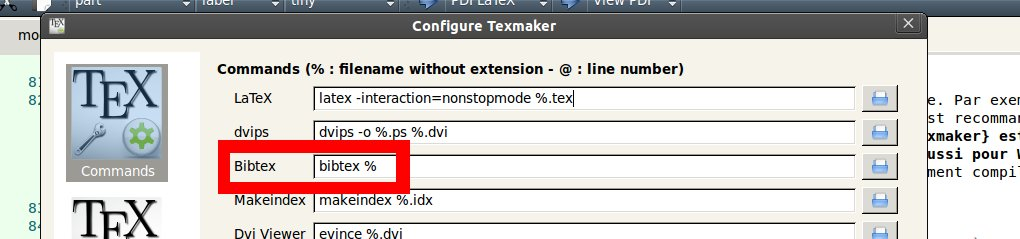
\includegraphics[scale=0.4]{images/bibtex.jpg}}
	% La commande '\caption' permet de définir la légende de la figure (obligatoire).
	% L'option entre crochets ([texte]) est une version courte de la légende, utilisée pour générer la liste des figures.
	\caption{Il est nécessaire de modifier l'option de BibTeX dans Texmaker.}
	% La commande '\label' donne un nom à la figure, et permet d'y faire référence dans le texte, 
	% grace à la commande '\ref', déjà utilisée précédemment.
	\label{fig:bibtex}
\end{figure}

Vous devez ensuite configurer Texmaker pour qu'il utilise le dictionnaire français lors de la vérification orthographique. Allez dans \textit{Options / Configure Texmaker / Editor / Spelling Dictionnary} et cliquez sur le bouton pour sélectionner le fichier \texttt{fr\_FR.dic} (c\@.f\@. figure \ref{fig:dictionnaire}). Si ce fichier n'est pas disponible, vous devez installer depuis le gestionnaire de packages ou MiKTeX un package dont le nom est du type \texttt{myspell-fr}. Une fois le dictionnaire sélectionné dans Texmaker, les fautes d'orthographes seront soulignées en rouge. Attention, le logiciel ne détecte pas les fautes de grammaire ou d'accord (genre, pluriel, conjugaison...). Soyez-donc attentifs à ce type d'erreurs !

\begin{figure}[htb]
	\centering
	\fbox{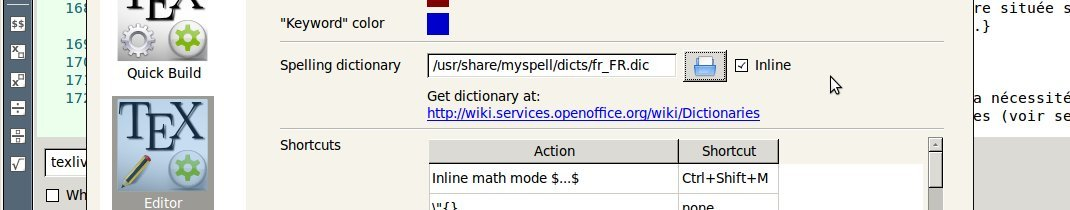
\includegraphics[scale=0.4]{images/dictionnaire.jpg}}
	\caption{Configuration du dictionnaire utilisé par le vérificateur d'orthographe.}
	\label{fig:dictionnaire}
\end{figure}

Pour pouvoir générer directement un fichier PDF, vous devez sélectionner le compilateur approprié. Dans la barre d'outil de Texmaker, cliquez sur \textit{LaTeX} et sélectionnez à la place \textit{PDFLaTeX}. Quand vous aurez besoin de compiler un document avec BibTeX (cf. section \ref{sec:biblio}), procédez de la même manière avec l'option BibTeX.

\subsection{Compilation}
Texmaker facilite grandement la création de documents \LaTeX{}. Il faut d'abord créer un nouveau fichier, y écrire le code source \LaTeX{} et l'enregistrer. Un exemple de code minimal est donné ci-dessous, que vous pouvez utiliser pour tester votre installation :
% Cette commande \vspace permet d'insérer un espace. On l'utilise ici pour bien
% séparer le paragraphe précédent de l'exemple.
% N'utilisez pas cette commande dans vos rapports ! Laissez LaTeX se
% charger de faire la mise en page tout seul.
\vspace{0.3cm}\\
\noindent{}\texttt{\textbackslash{}documentclass\{article\}}\\
\noindent{}\texttt{\textbackslash{}begin\{document\}}\\
\indent{}\texttt{Ceci est un document.}\\
\noindent{}\texttt{\textbackslash{}end\{document\}}
\vspace{0.3cm}

Il suffit ensuite de cliquer sur la flèche située à gauche de \textit{PDFLaTeX} dans la barre d'outils de Texmaker, comme indiqué dans la figure \ref{fig:compilation}, pour lancer la compilation du document. Vous pouvez également tester votre installation sur le fichier \texttt{.tex} fourni avec ce document : vous devez obtenir exactement le même PDF, puisqu'il a été généré de cette façon.

\begin{figure}[htb]
	\centering
	\fbox{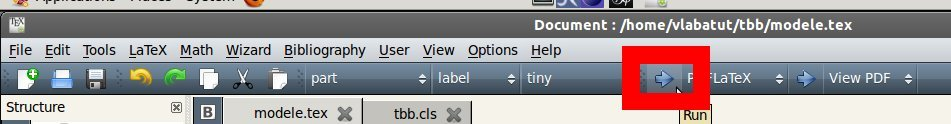
\includegraphics[scale=0.4]{images/compilation.jpg}}
	\caption{Le fait de cliquer sur la flèche indiquée déclenche la compilation du document \LaTeX{}.}
	\label{fig:compilation}
\end{figure}

Si la compilation rencontre des erreurs, celles-ci seront affichées dans la fen\^etre \textit{Messages / Log File} située en bas de Texmaker (figure \ref{fig:log}). Sinon, vous pourrez visualiser le document PDF en cliquant sur la flèche située à gauche de \textit{View PDF} (dans la barre d'outils). Si, lors lors du premier test, le compilateur ne trouve pas le fichier de classe \texttt{ceri.cls}, vérifiez que vous l'avez bien placé dans le même dossier que votre fichier \texttt{.tex}.

\begin{figure}[htb]
	\centering
	\fbox{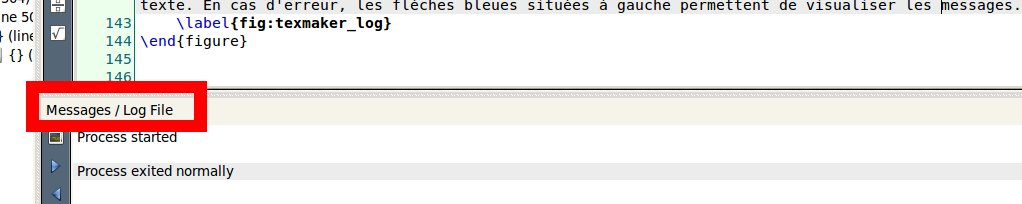
\includegraphics[scale=0.4]{images/log.jpg}}
	\caption{Texmaker affiche le résultat de la compilation dans la fen\^etre située sous l'éditeur de texte. En cas d'erreur, les flèches bleues situées à gauche permettent de visualiser les messages.}
	\label{fig:log}
\end{figure}

A noter qu'il est possible que le compilateur indique à l'aide d'un avertissement (warning) la nécessité de compiler une autre fois le document. C'est notamment le cas si des références bibliographiques ont été modifiées (voir section \ref{sec:biblio}) ou si la structure du document a changé (cf\@. section \ref{sec:structure}).

\subsection{Application Web}
Si vous ne voulez pas installer et configurer \LaTeX{} (ainsi que l'éditeur qui va avec) sur votre système, vous pouvez à la place vous tourner vers une application Web du type \href{https://www.overleaf.com/signup?ref=d62cb1694be6}{OverLeaf}. Vous devez d'abord vous créer un compte (c'est gratuit), puis vous pourrez définir et compiler vos propres documents en ligne. 

Notez que le source \LaTeX{}  du présent document est disponible sur OverLeaf à l'adresse : \url{https://www.overleaf.com/latex/templates/modele-rapport-uapv/pdbgdpzsgwrt\#.Vo_iNvnhDmF}. Il s'agit d'un modèle à partir duquel vous pouvez instancier votre propre document.

L'inconvénient principal de l'application en ligne (par rapport à l'application locale) est que la compilation prend sensiblement plus de temps. Par contre, les avantages sont multiples :  pas d'installation requise, simplicité d'utilisation, utilisable sur la plupart des navigateur, etc. De plus, OverLeaf permet le travail collaboratif : partage de documents, suivi des modifications, gestion des versions, système de commentaires, etc. Différents tutoriels sont disponibles sur le site officiel.



%%%%%%%%%%%%%%%%%%%%%%%%%%%%%%%%%%%%%%%%%%%%%%%%%%%
%% Généralités
%%%%%%%%%%%%%%%%%%%%%%%%%%%%%%%%%%%%%%%%%%%%%%%%%%%
\section{Généralités}
Vous devez indiquer le titre du document grâce à la commande \texttt{\textbackslash{}title} définie en début de fichier. Les noms des auteurs sont à spécifier dans la commande \texttt{\textbackslash{}author}.
		
\subsection{Mise en forme de base}
\label{sec:miseenforme}
La mise en forme de base est décrite clairement dans les références déjà citées \cite{Wikibooks2010, Wikibooks2011}. Voici rapidement quelques éléments utiles (référez-vous au code source pour comprendre le fonctionnement de ces commandes).
	
Le texte peut être mis en \textbf{gras} avec \texttt{\textbackslash{}textbf} ou en \textit{italique} avec \texttt{\textbackslash{}textit}. Il est possible d'inclure des listes non-numérotées avec \texttt{\textbackslash{}begin\{itemize\}} et \texttt{\textbackslash{}item}, telles que :	
% La commande '\begin{itemize}' permet de définir une liste dont les éléments ne sont pas numérotés.
\begin{itemize}
	% chaque élément est défini avec la commande '\item'
	\item premier élément ;
	\item 2\ieme élément ;
	\item troisième élément.
	\begin{itemize}
		\item on peut aussi placer des sous-listes ;
		\begin{itemize}
			\item et rajouter encore d'autres niveaux ;
			\item etc.
		\end{itemize}
		\item on continue au niveau supérieur ;
	\end{itemize}
	\item et au niveau encore supérieur.
\end{itemize}

Ou bien des listes numérotées avec \texttt{\textbackslash{}begin\{enumerate\}}, comme :
% La commande '\begin{enumerate}' fonctionne de la meme façon qu'itemize, mais les éléments sont numérotés.
\begin{enumerate}
	% Comme pour itemize, chaque élément est défini avec la commande '\item'
	\item premier élément ;
	\item 2\ieme élément ;
	\item troisième élément.
	\begin{enumerate}
		\item là encore, on peut placer des sous-listes ;
		\item ça marche exactement pareil que pour les listes non-numérotées ;
		\begin{itemize}
			\item on peut même mélanger les deux types de listes comme ici ;
			\item et ici.
		\end{itemize}
	\end{enumerate}
\end{enumerate}
	
% La commande '\colorbox{couleur}' permet de modifier la couleur de fond du texte.
Il est aussi possible de placer un fond coloré derrière le texte avec la commande \texttt{\textbackslash{}colorbox\{couleur\}}. Pour les couleurs, vous pouvez soit utiliser le nom de la couleur en anglais, par exemple \colorbox{red}{\texttt{red}}, soit définir une couleur précise en utilisant des valeurs numériques.

\textbf{Remarque :} évitez au maximum les notes de bas de page (pas de commande \texttt{\textbackslash{}footnote}) : placez vos remarques directement dans le texte, entre parenthèses.

\subsection{Structure}
\label{sec:structure}
Pour créer des paragraphes séparés, vous devez sauter une ligne (voir le code source). La structure du document est définie en utilisant des commandes spécifiques. Par ordre de niveau décroissant, on a :
\begin{enumerate}
	\item \texttt{\textbackslash{}section\{Titre de la section de niveau 1\}}
	\item \texttt{\textbackslash{}subsection\{Titre de la section de niveau 2\}}
	\item \texttt{\textbackslash{}subsubsection\{Titre de la section de niveau 3\}}
	\item \texttt{\textbackslash{}paragraph\{Titre de la section de niveau 4\}}
	\item \texttt{\textbackslash{}subparagraph\{Titre de la section de niveau 5\}}
\end{enumerate}

Les deux derniers niveaux ne sont pas utilisés dans ce document, car ils n'y sont pas nécessaires. Pour l'exemple, les voici :
\subsubsection{Section de niveau 3}
(Il est nécessaire de mettre une section de niveau 3 entre la section de niveau 2 et celle de niveau 4, sinon une section factice de niveau 3 numérotée 0 sera automatiquement créée).
\paragraph{Section de niveau 4}
Le niveau 4 n'est pas vraiment une section mais plutôt un titre de paragraphe. Pour cette raison, le titre n'est pas sur une ligne séparée, mais il est directement placé dans le paragraphe concerné.
\subparagraph{Section de niveau 5}
Même chose pour le niveau 5 : on a un titre inséré en début de paragraphe.
	
\textbf{Remarques :} ne définissez pas une section seulement pour y placer 1 ou 2 lignes de texte. Une section doit avoir un contenu assez long, sinon ce n'est pas la peine d'en créer une.
	
\subsection{Références croisées}
\label{sec:references}
\LaTeX{} permet de définir un label pour marquer un endroit particulier du document. Il est ensuite possible de faire référence à ce label. La référence apparaîtra dans le texte sous la forme d'un lien hypertexte, ce qui est pratique pour naviguer dans le document. 
	
Un label se définit avec la commande \texttt{\textbackslash{}label\{nomlabel\}} et une référence à un label avec \texttt{\textbackslash{}ref\{nomlabel\}}. Si le label correspond à un objet numéroté (figure, section, table...), alors c'est son numéro qui sera affiché.
	
La convention veut qu'on utilise des préfixes spécifiques dans les noms des labels en fonction du type d'objet référencé. Vous devez utiliser cette convention dans vos rapports (voir la table \ref{tab:prefixes}).
	
% La commande '\begin{table}' permet d'insérer une table dans le document.
% Elle fonctionne plus ou moins comme '\figure', notamment en ce qui concerne
% son positionnement avec h, t et b.
\begin{table}[htb]
	% La commande '\centering' sert encore à centrer la table.
	\centering
	% Cette commande permet de colorer une ligne sur deux, pour améliorer la visibilité
	\rowcolors{1}{LightColor}{}
	% La commande '\tabular' créé la table proprement dite.
	% le paramètre liste les colonnes de la table. Chaque lettre représente une colonne
	% et son alignement : l=alignée à gauche, r=alignée à droite et c=centrée.
	% Ici, on a deux colonnes alignées à gauche.
	\begin{tabular}{l l}
		\hline
		% La commande '\rowcolor' colorie la ligne de titre de couleur plus foncée.
		\rowcolor{DarkColor} 
		% Le contenu de la table est défini ligne à ligne. Les colonnes
		% sont séparées par le caractère '&' et la fin de la ligne est 
		% indiquée par la chaine '\\' (obligatoire).
		% La ligne de titre doit etre en gras (commande '\textbf')
		\textbf{Type d'objet}	& \textbf{Préfixe}	\\
		% La commande '\hline' insère une séparation d'épaisseur normale.
		\hline
		section					& \texttt{sec}	\\
		figure 					& \texttt{fig}	\\
		table 					& \texttt{tab}	\\
		equation 				& \texttt{eq}	\\
		\hline
	\end{tabular}
	% La légende est définie comme pour une figure.
	\caption{Préfixes utilisés conventionnellement pour définir les noms des labels.}
	% Le label aussi est défini comme pour une figure, mais en utilisant le préfixe 'tab' plutot que 'fig'.
	\label{tab:prefixes}
\end{table}
	
Il est absolument obligatoire que tout objet (équation, table, figure...) numéroté soit cité dans votre texte. Donc chacun doit avoir son label, et ce label doit apparaitre au moins une fois dans le texte. Bien sà»r vous ne devez pas vous contenter de citer chaque objet : ils doivent être suffisamment décrits, et de façon précise. Un objet qui n'est pas mentionné dans le texte ne sert à rien.



%%%%%%%%%%%%%%%%%%%%%%%%%%%%%%%%%%%%%%%%%%%%%%%%%%%
%% Objets
%%%%%%%%%%%%%%%%%%%%%%%%%%%%%%%%%%%%%%%%%%%%%%%%%%%
\section{Objets}
\label{sec:objets}
\LaTeX{} permet d'insérer un certain nombre d'objets numérotés : tables, équations, figures et algorithmes. Ces objets doivent toujours posséder une légende (sauf les équations) et être numérotés. De plus, ils doivent être mentionnés, décrits et commentés dans le texte. Toute référence à un objet doit être faite en utilisant la commande \texttt{\textbackslash{}ref\{nomlabel\}} (cf\@. section \ref{sec:references}).
	 
\LaTeX{} se charge de placer les objets dans le document. Il est possible de restreindre le positionnement en précisant si on veut que l'objet en question soit placé à l'endroit où il se trouve dans le document original (\texttt{h} pour \textit{here}), en haut de page (\texttt{t} pour \textit{top}) ou en bas de page (\texttt{b} pour \textit{bottom}). Il est possible de combiner ces valeurs si on veut donner plus de liberté au compilateur (ce qui est recommandé). Il est aussi possible que le compilateur place les objets ailleurs s'il est impossible de les placer à l'endroit spécifié.
	
En plus du positionnement, les légendes sont également gérées de façon automatique. Elles sont déclarées dans les objets, à l'aide de la commande \texttt{\textbackslash{}caption\{légende\}}.
	
\subsection{Tables}
\label{sec:tables}
La syntaxe permettant de définir des tables en \LaTeX{} est relativement compliquée. Vous vous limiterez à des tables de la forme décrite dans cette sous-section : cette mise en forme doit être respectée, afin de garder des tables lisibles. La commande \texttt{\textbackslash{}begin\{table\}[position]} permet d'insérer une table dans le document. Le paramètre \texttt{position} correspond à une combinaison de \texttt{h}, \texttt{t} et \texttt{b} qui permettra au compilateur de placer la table dans le document. Comme indiqué auparavant, le mieux est d'utiliser les trois, c'est à dire \texttt{htb}.
	
Chaque table doit être centrée, ce qui est réalisé avec la commande \texttt{\textbackslash{}centering}. La première ligne de la table contient les titres des colonnes. Le texte contenu dans cette ligne de titre doit être en \textbf{gras}. Les traits de séparation sont dessinées avec \texttt{\textbackslash{}hline}.
	
Le contenu proprement dit de la table est défini grâce à la commande \texttt{\textbackslash{}begin\{tabular\}\{colonnes\}}. Le paramètre \texttt{colonnes} permet de préciser à la fois le nombre de colonnes contenues dans la table, et leur alignement : 
\begin{itemize}
	\item \texttt{l} (\textit{left}) pour une colonne alignée à gauche ;
	\item \texttt{r} (\textit{right}) pour qu'elle soit alignée à droite ;
	\item \texttt{c} (\textit{center}) pour qu'elle soit centrée.
\end{itemize}

Les données de la table sont ensuite décrites ligne par ligne : la valeur de chaque colonne est séparée par un caractère \texttt{\&} et la fin de la ligne est marquée par un \texttt{\textbackslash{}\textbackslash{}} (obligatoire).
	
Vos tables doivent ressembler exactement à celles données en exemple dans ce document : couleurs, séparations, légende située en-dessous, etc. Les valeurs numériques doivent être alignées à droite. Les réels doivent être définis de manière à avoir le même nombre de décimales. Les valeurs textuelles peuvent être alignées à droite ou à gauche, ou bien centrées. Il est possible d'insérer des équations en-ligne (i\@.e\@. non-numérotées) dans une table (voir la section \ref{sec:equations}). La table \ref{tab:exemple} constitue un autre exemple à prendre en compte.
	
\begin{table}[htb]
	\centering
	\rowcolors{1}{LightColor}{}
	\begin{tabular}{l c r r c}
		\hline
		\rowcolor{DarkColor} 
		\textbf{Texte} 			& \textbf{Texte}			& \textbf{Entiers}	& \textbf{Réels}	& \textbf{Formules}	\\ 
		\hline
		% Le caractère '$' est un délimiteur permettant de passer dans le mode mathématique.
		% Le texte situé entre les '$' est interprété comme une formule mathématique et
		% est mis en forme de façon spécifique.
		Blabla bla bla bla bla	& Blabla bbla bla			& 21 				& 12,62				& $a+b=c$								\\
		Blabla bla bla bla		& Blabla bla bla bla bla	& 12356 			& 3456,21			& $x\cos{x}$							\\
		Blabla bla bla			& Blabla bla bbla bla		& 1 				& 45,87				& $\frac{\alpha^{2}+\beta}{\gamma}$	\\
		Blabla blabla bla bla	& Blabla bla bla bla		& 456 				& 45,16				& $\sqrt{x+y}$	\\
		Blabla bla blaa bla		& Blabla bla bla bla		& 78 				& 89,28				& $x_{1}-x_{2}$	\\
		Blabla bla bla bla bla	& Blabla bla bla bla		& 416 				& 10,10				& $\max_{x}{x}$	\\
		Blabla b bla bla		& Blabla blbla bla bla		& 9635 				& 99,99				& $\frac{x}{y}$	\\
		Blabla bla bbla bla		& Blabla bla b				& 965801 			& 46465,45			& $\Sigma_{x=1}^{10}{xy}$	\\
		Blabla bla				& Blabla bla				& 7 				& 48,78				& $\varphi^2$	\\
		\hline
	\end{tabular}
	\caption{Exemple de table contenant du texte, des valeurs entières, réelles et des formules mathématiques.}
	\label{tab:exemple}
\end{table}

Si votre table est haute et étroite, alors vous devez la décomposer afin de mieux utiliser l'espace. Ceci est illustré avec la table \ref{tab:etroit}, qui contient $50$ lignes pour seulement $2$ colonnes. Ceci est réalisé en utilisant l'environnement \texttt{minipage}, cf. le code source de ce document.
	
\begin{table}[htb]
	\rowcolors{1}{LightColor}{}
	% Chaque partie de la table doit être placée dans un environnement "minipage".
	% Ici, le paramètre "0.19\linewidth" indique que la première partie de la table
	% occupe 19% de la largeur de la page. Il faut donc adapter cette valeur en
	% fonction du nombre de parties à afficher.
	\begin{minipage}[t]{0.19\linewidth}
		\centering
		\begin{tabular}{l l}
			\hline
			\rowcolor{DarkColor} 
			\textbf{Col1} 			& \textbf{Col2} \\ 
			\hline
			1 & hdc \\
			2 & orf \\
			3 & seh \\
			4 & lig \\
			5 & jhg \\
			6 & azr \\
			7 & opi \\
			8 & hgj \\
			9 & xvc \\
			10 & ree \\
			\hline
		\end{tabular}
	\end{minipage}
	% Deuxième partie de la table...
	\begin{minipage}[t]{0.19\linewidth}
		\centering
		\begin{tabular}{l l}
			\hline
			\rowcolor{DarkColor} 
			\textbf{Col1} 			& \textbf{Col2} \\ 
			\hline
			11 & ytr \\
			12 & xcv \\
			13 & fsd \\
			14 & pui \\
			15 & gsf \\
			16 & aze \\
			17 & bcv \\
			18 & wxc \\
			19 & uyr \\
			20 & ndz \\
			\hline
		\end{tabular}
	\end{minipage}
	% Troisième partie de la table...
	\begin{minipage}[t]{0.19\linewidth}
		\centering
		\begin{tabular}{l l}
			\hline
			\rowcolor{DarkColor} 
			\textbf{Col1} 			& \textbf{Col2} \\ 
			\hline
			21 & ioe \\
			22 & snu \\
			23 & dgp \\
			24 & zbu \\
			25 & zvz \\
			26 & orv \\
			27 & czr \\
			28 & azh \\
			29 & cyh \\
			30 & ytj \\
			\hline
		\end{tabular}
	\end{minipage}
	% Quatrième partie de la table...
	\begin{minipage}[t]{0.19\linewidth}
		\centering
		\begin{tabular}{l l}
			\hline
			\rowcolor{DarkColor} 
			\textbf{Col1} 			& \textbf{Col2} \\ 
			\hline
			31 & zyc \\
			32 & opv \\
			33 & azv \\
			34 & xdf \\
			35 & yzd \\
			36 & sgg \\
			37 & sss \\
			38 & zdv \\
			39 & sgu \\
			40 & vzd \\
			\hline
		\end{tabular}
	\end{minipage}
	% Cinquième partie de la table...
	\begin{minipage}[t]{0.19\linewidth}
		\centering
		\begin{tabular}{l l}
			\hline
			\rowcolor{DarkColor} 
			\textbf{Col1} 			& \textbf{Col2} \\ 
			\hline
			41 & oze \\
			42 & anb \\
			43 & kir \\
			44 & sfk \\
			45 & bed \\
			46 & pyj \\
			47 & zdj \\
			48 & pyj \\
			49 & zen \\
			50 & oef \\
			\hline
		\end{tabular}
	\end{minipage}
	\caption{Exemple de table haute et étroite, décomposée en 5 parties pour occuper plus efficacement l'espace disponible.}
	\label{tab:etroit}
\end{table}

\subsection{Équations}
\label{sec:equations}
Les équations peuvent être introduites sous deux formes : \textit{en}-ligne et \textit{hors}-ligne. Une équation en-ligne est intégrée au texte, par exemple $y=ax+b$. La syntaxe \LaTeX{} consiste simplement à l'entourer avec des caractères \texttt{\$} : le 1\ier~\texttt{\$} active ce qu'on appelle le \textit{mode mathématique} et le 2\ieme~le désactive. Le texte situé entre les deux est interprété de façon différente du texte normal. Voyez \cite{Wikibooks2010, Wikibooks2011} pour plus de détails sur les nombreuses possibilités de \LaTeX{} en ce qui concerne les formules mathématiques, et le code source de la table \ref{tab:exemple} pour quelques exemples. Cette méthode permet aussi d'insérer des formules dans les tables, comme par exemple dans la table \ref{tab:exemple}.

% La commande '\begin{equation}' permet de définir une équation hors-ligne.
% On ne donne pas de légende aux équations, et il est inutile de les centrer
% (elles le sont par défaut). On ne peut pas les positionner non plus (elles
% apparaissent là où elles sont définies).
\begin{equation}
	f(s)=h(s)+g(s)
   	% Par contre, si on veut faire référence à l'équation, il est nécessaire
   	% d'y définir un label.
	\label{eq:exemple}
\end{equation}

Les équations hors-ligne sont séparées du texte et numérotées. En y associant un label, il est donc possible d'y faire référence dans le texte. Par exemple, l'équation ci-dessus est l'éq. \ref{eq:exemple}. On les définit en utilisant la commande \texttt{\textbackslash{}begin\{equation\}}. Une équation n'a pas de légende, et elle doit être décrite dans le texte qui y fait référence.

\textbf{Remarques :}
\begin{itemize}
	\item Vos variables et fonctions doivent avoir des noms courts : une lettre et un indice, maximum. Pas de nom du type ${mafonction}$, mais plutôt $f$, $f'$ $f_1$, etc\@.
	\item Ne mélangez pas les notations informatiques et mathématiques. Par exemple n'utilisez pas la notation tableau (array), comme par exemple \texttt{tab[12]}, dans une équation.
\end{itemize}
	
	
\subsection{Figures}
\label{sec:figures}
Une figure s'insère de manière très similaire à une table, excepté qu'on utilise la commande \texttt{\textbackslash{}begin\{figure\}} au lieu de \texttt{\textbackslash{}begin\{table\}}. A part ça, la commande \texttt{\textbackslash{}centering} doit toujours être présente pour centrer la figure, la légende doit être définie en-dessous de la figure avec \texttt{\textbackslash{}caption}, et un label peut être créé avec \texttt{\textbackslash{}label} pour référencer la figure, comme par exemple la figure \ref{fig:bibtex}.

\begin{figure}[th]
	\centering
	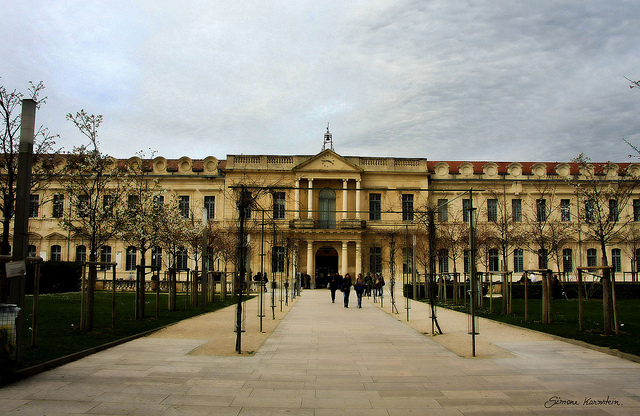
\includegraphics[scale=0.5]{images/univ.jpg}
	\caption{L'université d'Avignon.}
	\label{fig:uapv}
\end{figure}

L'utilisation du compilateur \textit{PDFLaTeX} permet de traiter seulement des fichiers aux formats PNG, JPEG, GIF et PDF. L'image est spécifiée au moyen de la commande \texttt{\textbackslash{}includegraphics[scale=s]\{fichier\}}, où \texttt{fichier} est le chemin du fichier contenant l'image (les chemins relatifs sont exprimés par rapport à l'emplacement du fichier \texttt{.tex} en cours de compilation) et \texttt{s} est une valeur réelle indiquant l'échelle de l'image (optionnel). A la place du paramètre \texttt{scale}, vous pouvez spécifier la largeur ou la hauteur de l'image, par exemple avec \texttt{width=12cm} ou \texttt{height=5cm}.

Tous les algorithmes doivent être donnés sous forme de diagrammes du genre \href{http://en.wikipedia.org/wiki/Flowchart}{flowchart} \cite{Wikipedia2011}, qui apparaîtront dans le rapport en tant que figures. Il faut éviter à tout prix le pseudo-code. 



%%%%%%%%%%%%%%%%%%%%%%%%%%%%%%%%%%%%%%%%%%%%%%%%%%%
%% Références
%%%%%%%%%%%%%%%%%%%%%%%%%%%%%%%%%%%%%%%%%%%%%%%%%%%
\section{Références bibliographiques}
\label{sec:biblio}
Le système \LaTeX{} peut être couplé avec BibTeX afin de gérer automatiquement les références bibliographiques du document. La procédure consiste d'abord à définir un fichier de type BibTeX décrivant chaque référence en détails. Comme indiqué précédemment, il est recommandé d'utiliser un logiciel spécifique comme \href{http://jabref.sourceforge.net/}{JabRef} \cite{JabRef2008} pour réaliser cette tâche. Le fichier \texttt{bibliographie.bib} fourni avec ce document est un exemple de fichier BibTeX. Il est placé dans le même dossier que le fichier \texttt{.tex} à compiler.

Une référence bibliographique doit toujours indiquer au moins les auteurs, le titre du document et l'année de publication. Dans un contexte académique, une référence vers un article de journal scientifique, comme \cite{Fortunato2010} par exemple, doit également contenir le nom du journal, le volume, le numéro et les pages. Pour une conférence, comme par exemple \cite{Wei1989}, les champs additionnels sont le nom de la conférence et les pages. Pour un rapport technique comme \cite{Rosvall2009a} ou une thèse comme \cite{Gerbaud2010}, il faut aussi indiquer l'institution d'affiliation des auteurs.

Dans le fichier \texttt{.tex}, une référence est introduite au moyen de la commande \texttt{\textbackslash{}cite\{cle\}}, où \texttt{cle} est la clé associée dans le fichier BibTeX à la référence désirée. Par exemple la commande \texttt{\textbackslash{}cite\{Wikibooks2010\}} permet d'introduire la citation suivante : \cite{Wikibooks2010}. Il faut ensuite compiler le document avec BibTeX (voir la section \ref{sec:installation}), puis le recompiler avec PDFLaTeX.
	
Attention, lorsque vous définissez une clé n'utilisez pas de caractères accentués. Vous pouvez mettre plusieurs références dans une même commande \texttt{\textbackslash{}cite}, par exemple \texttt{\textbackslash{}cite\{Wikibooks2010, Wikibooks2011\}} donne \cite{Wikibooks2010, Wikibooks2011}.
	
BibTeX et \LaTeX{} vont s'occuper de numéroter les références automatiquement. La commande \texttt{\textbackslash{}bibliography\{fichier\}} permet d'insérer une liste des références, généralement on la place à la fin du document. Le paramètre \texttt{fichier} doit indiquer l'emplacement et le nom du fichier BibTeX à utiliser. Pour vous aider, le fichier \texttt{bibliographie.bib} est fourni à titre d'exemple.
	
Toutes les informations que vous intégrez à votre rapport et qui n'ont pas été produites par vous-même doivent être explicitement référencées. Vous devez donc indiquer tout document que vous utilisez, y compris ce qui est récupéré sur internet. Cela vaut pour tout type d'information : document texte, images, vidéos, code source, algorithmes, idées diverses.

Autrement dit, vous avez le droit de réutiliser absolument tout ce que vous désirez. Par contre, vous devez à chaque fois indiquer exactement ce que vous réutilisez, et à qui/où vous l'avez pris. De plus, vous devez expliquer ce que vous avez modifié (par exemple s'il s'agit d'un algorithme) et la nature de ces modifications.



  
%%%%%%%%%%%%%%%%%%%%%%%%%%%%%%%%%%%%%%%%%%%%%%%%%%%
%% Conclusion
%%%%%%%%%%%%%%%%%%%%%%%%%%%%%%%%%%%%%%%%%%%%%%%%%%%
\section{Conclusion}
Avec \LaTeX{} on obtient un rendu impeccable mais il faut s'investir un minimum pour le prendre en main. Pensez à consulter le code source de ce document, qui est abondamment commenté.
 
 
  
  
%%%%%%%%%%%%%%%%%%%%%%%%%%%%%%%%%%%%%%%%%%%%%%%%%%%
%% Bibliographie
%%%%%%%%%%%%%%%%%%%%%%%%%%%%%%%%%%%%%%%%%%%%%%%%%%%
\MyBibliography{bibliographie}


\end{document}

